\chapter{Diseño e implementación}

\label{Chapter3}

En el presente capítulo se presentan los detalles del diseño y los criterios adoptados para el desarrollo del trabajo junto con los pasos seguidos para la implementación del mismo.

\section{Arquitectura del sistema}

La arquitectura del sistema es de cliente-servidor. Está constituido por dos nodos y un servidor, los cuales están conectados a la red local y se comunican a través del protocolo MQTT. De esta forma el servidor recibe los parámetros actuales de estado y cambios desde cada dispositivo, los procesa y almacena en la base de datos. También envía mensajes hacia los dispositivos para cambiar el estado de las salidas o el parámetro que se desee cambiar. Los usuarios pueden consultar y modificar el estado de los dispositivos desde un navegador web móvil o desde una computadora.

En la imagen \ref{fig:9} se puede observar una arquitectura típica cliente-servidor implementada con una Raspberry Pi.

\begin{figure}[h]
\centering
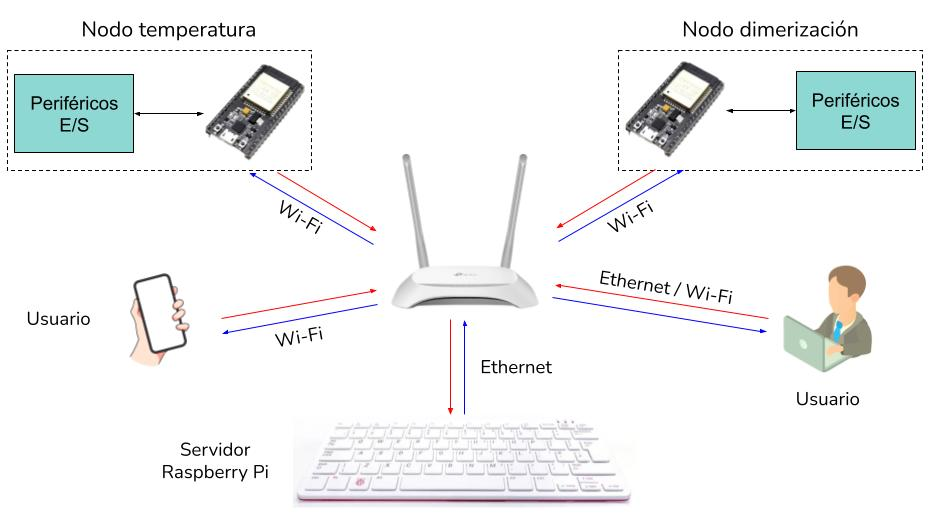
\includegraphics[scale=1.4]{Imagen 9 - cliente-servidor.jpg}
\caption[Arquitectura cliente-servidor]{Arquitectura cliente-servidor. \footnotemark}
\label{fig:9}
\end{figure}
\footnotetext{Imagen tomada de: \url{https://www.bujarra.com/raspberry-pi-servidor-vpn-con-pptp/}}

Uno de los nodos tiene como función sensar y controlar de temperatura de un recinto, y el otro controlar la iluminación. Originalmente el proyecto estaba pensado para que un solo nodo implemente estas dos funciones, pero durante el desarrollo se optó por la implementación separada. Este cambio se basó en la idea de modularizar los nodos y que sus funciones sean específicas. De esta forma es más amigable para el usuario visualizar y modificar el estado en pantalla e implementar el alta de nuevos dispositivos en el sistema.

El servidor está montado sobre una Raspberry Pi 400 con un sistema operativo Raspbian con interfaz gráfica. Este sistema operativo es la versión oficial ofrecida por la fundación Rasperry Pi y está basado en Debian versión 11 (\textit{bullseye}). En esta etapa de desarrollo se optó por una Raspberry Pi 400 por una cuestión de costos y practicidad a la hora de desarrollar y hacer las pruebas, aunque tiene un mayor volumen que los otros modelos de la familia. Al momento de ofrecer una solución definitiva está pensado que sea implementado en una placa con el formato más pequeño como cualquiera de las Raspberry Pi 4. La conexión del servidor a la red local es por cable ethernet.

\subsection{Especificaciones técnicas del servidor}

El sistema operativo del servidor está instalado y se ejecuta desde un disco de estado sólido por USB, que tiene una mayor capacidad de escrituras y lecturas que una memoria microSD. Esto favorece al momento de hacer pruebas en un desarrollo de este estilo.  El sistema operativo y todo el software adicional tendría que estar montado en una tarjeta SD para que todo el conjunto sea lo más pequeño posible.

En la tabla \ref{tab:Especificaciones Raspberry Pi 400} pueden verse las especificaciones técnicas de hardware más importantes del modelo Raspberry Pi 400.

\begin{table}[h]
\centering
\caption[Raspberry Pi 400]{Especificaciones de Raspberry Pi 400.}
\begin{tabular}{l c}
\toprule
Procesador		&	Broadcom BCM2711 quad-core Cortex-A72(ARM v8) \\
				&	64-bit SoC @ 1.8GHz \\
\midrule
Memoria			&	4GB LPDDR4-3200 \\
\midrule
				&	2.4GHz and 5.0GHz 802.11b/g/n/ac wireless LAN \\
Conectividad		&	Bluetooth 5.0, BLE\\
				&   Gigabit Ethernet \\
\midrule
Alimentación		&	5V DC vía USB-C\\
\bottomrule
\hline
\end{tabular}
\label{tab:Especificaciones Raspberry Pi 400}
\end{table}

\section{Modelo de datos}



\section{Desarrollo del frontend}



\section{Desarrollo del backend}



\section{Nodos, sensores y actuadores}



\section{Comunicación del sistema}